%-----------------------------------------------------------------------------
%  Copyright (C) 2004-2017 Andrew Mathas, University of Sydney
%
%  Distributed under the terms of the GNU General Public License (GPL)
%                  http://www.gnu.org/licenses/
%
% This file is part of the MathQuiz system.
%
% <Andrew.Mathas@sydney.edu.au>
%-----------------------------------------------------------------------------

\synctex=1

\PassOptionsToClass{tikz,svgnames}{xcolor}
\documentclass[svgnames]{article}
\usepackage[a4paper,margin=30mm]{geometry}
\parindent=4mm
\parskip=1mm
\hfuzz 5pt

\usepackage{pdfpages}
\usepackage{etoolbox}% to patch l@section to remove extraneous spacing
\def\sectionautorefname{Chapter}
\def\subsectionautorefname{Section}

\usepackage[nonewpage]{imakeidx}
\indexsetup{level=\section*,toclevel=section,noclearpage}
\makeindex[intoc,noautomatic]
\indexprologue{\textit{This is an index only for the main \MathQuiz manual. It does not index
the on-line manual.}}

\usepackage{mathquiz-doc}

\setcounter{secnumdepth}{2}
\setcounter{tocdepth}{3}
% automatic indexing using quotes: "word" puts word in the index and
% typsets it as \Verb|Word|.
\catcode`\"=13
\def"#1"{\Verb|#1|\index{#1}}
\newcommand\lowerCaseIndex[1]{%
  \lowercase{\def\temp{#1}}%
  \expandafter\index\expandafter{\temp@#1}%
}
% usage: \CrossIndex[*]{main entry}[*]{subentry} with *'s for macros
\NewDocumentCommand\CrossIndex{ smsm }{%
  \IfBooleanTF{#1}{%
    \lowercase{\def\tempa{#2}}%
    \xdef\tempa{\tempa@\noexpand\textbackslash#2}%
  }{\def\tempa{#2}}%
  \IfBooleanTF{#3}{%
    \lowercase{\def\tempb{#4}}%
    \xdef\tempb{\tempb@\noexpand\textbackslash#4}%
  }{\def\tempb{#4}}%
  \expandafter\index\expandafter{\tempa!\tempb}%
  \expandafter\index\expandafter{\tempb}%
}
\newcommand\macroIndex[1]{%
  \lowercase{\def\temp{#1}}%
  \expandafter\index\expandafter{\temp@\textbackslash#1}%
}

\newif\ifCtan\Ctanfalse % condition compilation for ctan distribution

\renewcommand*\contentsname{\relax}

% hyperref links to ctan
\NewDocumentCommand\ctan{ O{pkg/#2} m}{\href{https://www.ctan.org/#1}{\texttt{#2}}}

\newcommand\ddash{\texttt{\textemdash\textemdash}}
\newcommand\mathquizopt[1]{\textsf{mathquiz \ddash#1}}

%%%%%%%%%%%%%%%%%%%%%%%%%%%%%%%%%%%%%%%%%%%%%%%%%%%%%%%%%%%%%%%%%%%%%%%%%%%%%%%%%%%%%%%
%% MathQuiz title box for front page
\usepackage{tikz}
\usetikzlibrary{shadows.blur}

\definecolor{stone}{HTML}{E9E0D8}
\tikzset{shadowed/.style={blur shadow={shadow blur steps=5},
                          top color=stone,
                          bottom color=PapayaWhip,
                          draw=SaddleBrown,
                          shade,
                          font=\normalfont\Huge\bfseries\scshape,
                          rounded corners=8pt,
      },
      boxes/.style={draw=Sienna,
                    fill=Cornsilk,
                    font=\sffamily\small,
                    inner sep=5pt,
                    rectangle,
                    rounded corners=8pt,
                    text=Brown,
     }
}

\def\MathQuizTitle{
  \begin{tikzpicture}[remember picture,overlay]
      \node[yshift=-3cm] at (current page.north west)
        {\begin{tikzpicture}[remember picture, overlay]
          \draw[shadowed](30mm,0) rectangle node[Brown]{MathQuiz} (\paperwidth-30mm,16mm);
          \node[Sienna,font=\normalfont\small\itshape] at (\paperwidth/2,2mm)
          {\small \mathquiz{description}};
          \node[anchor=west,boxes] at (4cm,0cm) {\mathquiz{name}};
          \node[anchor=east,boxes] at (\paperwidth-4cm,0) {Version \mathquiz{version}};
         \end{tikzpicture}
        };
   \end{tikzpicture}
}

\hypersetup{pdftitle={MathQuiz manual}}

%%%%%%%%%%%%%%%%%%%%%%%%%%%%%%%%%%%%%%%%%%%%%%%%%%%%%%%%%%%%%%%%%%%%%%%%%%%%%%%%%%%%%%%
%% headers and footers
\makeatletter
\def\@oddfoot{\tiny\MathQuiz -- \mathquiz{version}\hfill\thepage}
\patchcmd\l@section{1.0em}{0.5em}{}{}
\makeatother

\begin{document}

    \MathQuizTitle

    \begin{quote}
      \MathQuiz makes it possible to write on-line quizzes using
      \LaTeX, providing an easy way for anyone who knows \LaTeX\ to
      create an on-line quiz using \LaTeX\ file.  The
      allows the quiz author to concentrate on the content of quizzes,
      unencumbered by the technicalities of HTML and javascript.

      \ScreenShot{Example quiz}{examples/quiz-page}

      \begin{center}
        \vskip-10mm
        \begin{minipage}{0.7\textwidth}
          \hspace*{3em}\tableofcontents
        \end{minipage}
      \end{center}
    \end{quote}

    \newpage

\section{Introduction}
    On-line quizzes provide a good way to reinforce learning, especially
    because they can give ``interactive'' feedback to the students based
    on the answers that they give. Unfortunately, in addition to writing
    the quiz content there are significant technical hurdles that need
    to be overcome when writing an on-line quiz -- and there are
    additional complications if the quiz involves mathematics or
    diagrams.

    \MathQuiz makes it possible to write on-line quizzes using \LaTeX,
    which is the typesetting language used by mathematicians and
    educators use \LaTeX\ to write their research papers, books and
    teaching materials.  In principle, the quiz can contain anything
    that can be typeset using \LaTeX.  In practise, the \LaTeX\ is
    converted to HTML using
    \href{https://www.tug.org/applications/tex4ht/mn.html}{\TeX 4ht}
    (and \href{https://github.com/michal-h21/make4ht}{make4ht}), so the
    quizzes can contain any \LaTeX commands that are understood by \TeX 4ht,
    which is almost everything. In particular, it is possible to use
    graphics constructed using packages like \ctan{pstricks} and
    \ctan{tikz}.

    \MathQuiz supports the following three types of questions:
    \begin{itemize}
      \item Multiple choice questions with a unique correct answer
      \item Multiple choice questions zero or more correct answers
      \item Questions with a numerical answer.
    \end{itemize}
    Each time a student answers a question they are told whether they
    are right or wrong and it is possible for the quiz author to give
    targeted feedback to the student based on their answer.

    The easiest way to explain how \MathQuiz works is by example. The
    following \LaTeX\ file defines a quiz with a single multiple choice
    question that has four possible answers, each of which has a
    customised response.  (Responses to answers are optional, but they
    are one of the main pedagogical advantages of on-line quizzes
    because the quiz can explain to the student why their answer was
    correct or incorrect.)

    \lstinputlisting[style=latexcode]{examples/simple}

    Since this is a \LaTeX\ file it can be processed using
    \texttt{pdflatex}, or \texttt{latex}, to produce a readable and
    printable version of the quiz, which can be useful when
    proofreading. In this case, the \LaTeX\ version of the quiz looks
    something like this:

    \ScreenShot[0.5]{PDF page}{examples/simple-pdf}

    Of course, the real reason for using \MathQuiz is that it is also
    possible to make an on-line version of the quiz by processing the
    quiz using the \texttt{mathquiz} command. If you do this, and then open
    the resulting web page in your favourite browser, you will see a web page
    that looks something like this:

    \ScreenShot{Web page}{examples/simple-html}

    The on-line version of the quiz displays one question at a time,
    with the question buttons serving the dual purpose of, first,
    providing a way to navigate between the different questions in the
    quiz and, secondly, displaying whether or not the question has been
    attempted and, if so, whether it answered correctly or incorrectly.
    Targeted feedback can be given to the person taking the quiz based
    on their responses.

    As explained in \autoref{S:documentclass}, it is possible to
    customise some aspects of the web pages constructed by \MathQuiz.
    With some rudimentary knowledge of python, it is possible to change the page
    layout of the quizzes or to embed them into your local web pages; see
    \autoref{SS:customisation}.

\subsection{What MathQuiz does and does not do}

    The \MathQuiz program was designed to be run from the command-line,
    so to process the file \textsf{quiz.tex} using \MathQuiz you would
    type

    $>$ \Verb|mathquiz quiz| \qquad or \qquad $>$ \Verb|mathquiz quiz.tex|

    \noindent from the command-line. Although I have not tested this, it
    should also be possible to run \MathQuiz from inside programs like
    \TeX Shop by setting the compiler equal to \textsf{mathquiz}.

    \MathQuiz can be used to ask the student a series of questions. In
    the on-line version of the quiz, one question is displayed at a
    time. Each question in a quiz, and each quiz itself, can be
    attempted as many times as the student wants. \MathQuiz does not
    limit the number of times that questions can be attempted.
    The following three types of questions are supported:
    \begin{itemize}
      \item Multiple choice questions with a unique correct answer
      \item Multiple choice questions zero or more correct answers
      \item Questions with a numerical answer.
    \end{itemize}
    Questions with symbolic answers are not supported.
    For example, if the answer to a question is $0$ then $\sin(0)$ will
    not be accented as a correct answer and the only way to ask for the
    indefinite integral of a function is as a multiple choice question.

    The quizzes made using \MathQuiz are intended to be used as a
    revision resource rather than as an assessment tool. Consequently,
    \MathQuiz does not provide a mechanism for recording the marks
    obtained by the students taking the quiz. Technically, it probably
    would not be very hard to record marks but this introduces a
    significant amount of extra overhead in terms of student
    authentication and interfacing with a database. In addition, if
    \MathQuiz were used as an assessment tool then there would be
    additional ``security issues'' to ensure that the quiz content is
    secure. Currently, even though the solutions to the quiz questions
    do not appear in the HTML source code for the quiz it is possible to
    access the answers if you know when you are doing.

    The questions in a \MathQuiz quiz are static. In particular, they do
    not accept variables and exactly the same questions will appear in
    exactly the same order each time the quiz is taken. It would not be
    hard to make the questions appear in a random order. Randomising the
    order of the multiple choice answers would be more be difficult with
    the current implementation.

    The quizzes are not timed and do not have time-limits.

    Finally, the point pf \MathQuiz is to make it possible to write
    on-line quizzes without knowing any HTML, so \MathQuiz provides
    almost no mechanisms for controlling the style and format of the
    quizzes that it creates (although see \autoref{SS:customisation}).
    It is possible to add some styling using, for example, the
    \Verb|\Css| command from \ctan{tex4ht}, however, if you really want
    to do this then you are probably better off writing
    \href{https://www.w3schools.com/css/}{CSS} directly.

    Some of the ``missing features'' listed above may be added to \MathQuiz in a future release.

\subsection{Credits}
    \MathQuiz{} was written and developed in the
    \href{http://www.maths.usyd.edu.au/}{School of Mathematics and
    Statistics} at the \href{http://www.usyd.edu.au/}{University of
    Sydney}.  The system is built on \LaTeX{} with the conversion from
    \LaTeX{} to HTML being done by Eitan Gurari's
    \href{http://www.cis.ohio-state.edu/~gurari/TeX4ht/mn.html}{TeX4ht}
    and
    \href{https://github.com/michal-h21/make4ht}{make4ht}.

    To write quizzes using \MathQuiz it is only necessary to know
    \LaTeX, however, the underlying \MathQuiz system actually has three components:
    \begin{itemize}
      \item A \href{https://www.latex-project.org/}{\LaTeX} document class file, \texttt{mathquiz.cls}, and
      a \ctan[tex4ht]{\TeX 4ht} configuration file, \texttt{mathquiz.cfg}, that enable the
      quiz files to be processed by \LaTeX{} and \TeX 4ht, respectively.
      \item A \href{https://www.python.org/}{python} program, \texttt{mathquiz}, that translates the
      \LaTeX{} into xml, using \TeX 4ht, and then into HTML.
      \item \href{https://www.w3schools.com/Js/}{Javascript} and \href{https://www.w3schools.com/css/}{css}
      code that works behind the screens to control and style the quiz web pages.
    \end{itemize}

   The \LaTeX{} component of \MathQuiz{} was written by Andrew Mathas
   and the python, css and javascript code was written by Andrew Mathas
   (and Don Taylor), based on an initial prototype of Don Taylor's from
   2001.  Since 2004 the program has been maintained and developed by
   Andrew Mathas. Although the program has changed substantially since
   2004 some of Don's code and, in particular, his idea of using
   \TeX4ht are still very much in use.

   Thanks are due to Bob Howlett for general help with CSS and, for
   Version~5, to  Michal Hoftich for invaluable technical advice on
   \TeX4ht.

\section{System requirements, installation and configuration}
  \index{system requirements}
  \CrossIndex{system requirements}{tex4ht}
  \CrossIndex{system requirements}{make4ht}
  \CrossIndex{system requirements}{python}

  \subsubsection[System requirements: Python3, \LaTeX{} and \TeX4ht]%
          {System requirements: Python3 and \LaTeX, including \TeX 4ht
    and \textsc{make4ht}}

    It is advisable to have an up to date distribution of \LaTeX, such
    as that provided by \href{https://www.tug.org/texlive/}{\TeX live},
    as well as a recent version of \href{https://www.python.org/}{Python 3}
    (as of writing, python 3.6 is available). I have tested the
    \MathQuiz system extensively on linux and mac operating systems.
    The program should work under windows, however, I do not have access
    to window machine to test it on.

    \subsubsection{\MathQuiz components}

    The \MathQuiz program has different components:
      \begin{itemize}
           \item \LaTeX\ files (a class file and \TeX4ht configuration files)
           \item Python3 executables that use \TeX4ht to convert \LaTeX\ files into web pages
           \item Web files (javascript, css and on-line documentation)
           \item \LaTeX\ Documentation
      \end{itemize}
    In order for \MathQuiz to work all of these files need to be put in
    appropriate places. Of course, to use the on-line quizzes created by
    \MathQuiz you will also need a web server.  This section guides you
    through what needs to be done.
    \ifCtan
       Fortunately, because \MathQuiz is installed as part of your \TeX\
       distribution, you only need to install the web files used by \MathQuiz
       and this can be done using \MathQuiz.

    \else

    \subsubsection{Installation from the zip file}
      The \MathQuiz zip file has three directories, or folders:

      \begin{itemize}
        \item[--] mathquiz/latex
        \item[--] mathquiz/doc
        \item[--] mathquiz/scripts
      \end{itemize}

      The files in the \textsf{latex} directory need to be put somewhere in the \LaTeX\
    search path. For example, on my computer I have these files in

       \Verb|/usr/local/texlive/texmf-local/tex/latex/local/mathquiz|

    After you have moved these files to an appropriate place you will probably need to run
    something like texhash. The exact command that you need to run to tell
    \LaTeX\ that you have installed some files install the latex
    components of the system depends on the \TeX distribution that you are
    using.

    The files in the \textsf{doc} directory are the documentation. You can
    put these files where ever you like!

    The \MathQuiz program itself lives in the script directory. On a unix
    like system I recommend making a link to the file mathquiz.py, which is
    the entry point to the code, using something like:

        \Verb|ln -s <path to scripts directory>/mathquiz.py mathquiz|

    \noindent Of course, the \textsf{mathquiz} executable should be in the system path.

    It remains to install the web files used by \MathQuiz, which can be
    done using \MathQuiz.
    \fi

    \subsubsection{Installing the web files used by \MathQuiz}
    \index{installation}

     The quiz files created by \MathQuiz use
     \href{https://en.wikipedia.org/wiki/JavaScript}{javascript} and
     \href{https://www.w3schools.com/css/css_intro.asp}{cascading style
     sheets} (CSS) to render the quizzes. You do not need to understand
     how this works but you do need to put the \MathQuiz javascript and
     CSS files onto your web server.\footnote{In fact, \MathQuiz will work
     even if you do not install these files on your web server, however,
     the quiz pages that it creates will have an annoying message at the
     top of the web page that asks you to install these files.}  Rather
     than doing this by hand you need to do this using the following
     \MathQuiz command:

     $>$ \mathquizopt{initialise}

     \noindent This command will copying the files onto the web server
     and set up a configuration file so that \MathQuiz knows where these
     files are. These files can either be installed in a system directory,
     so that everyone can use them, or they can be put into you own web
     directories.

     When you run the \MathQuiz initialisation command you will be prompted for the
     following:
     \begin{itemize}
       \item The \MathQuiz web directory, which is a directory on your local file system that is visible
             from to your web server
       \item The \MathQuiz URL, which is the \textit{relative} URL to this
       directory that you use to access the files in this directory from
       your browser
     \end{itemize}
     For example, on my system the base directory for our web server is
     \textsf{/usr/local/httpd/} and the \MathQuiz web
     files are in \textsf{/usr/local/httpd/MathQuiz}. So, I set:
     \begin{quote}
       \begin{tabular}{lll}
         \MathQuiz web directory &=& \textsf{/usr/local/httpd/MathQuiz}\\
         \MathQuiz relative URL  &=& \textsf{/MathQuiz}
       \end{tabular}
     \end{quote}
     In addition, you can set global defaults for the following.
     \begin{itemize}
       \item department = a (short) name for your department
       \item department\_url = the URL for your department web server
       \item institution = a (short) name for your institution
       \item institution = the URL for your institution
     \end{itemize}
    Leave these blank if you do not want to set defaults for the department and
    institution. You can change these settings at any time using\quad
    \mathquizopt{edit-settings}. You can also set these in the \LaTeX\ file
    for the quiz.

    \bigskip

    \MathQuiz is now ready to use!

  \section{The MathQuiz document class (the \LaTeX{} commands)}\label{S:documentclass}

  This section describes the commands and environments provided by the
  \MathQuiz document class. The aim of \MathQuiz is to construct web
  pages for quizzes the \LaTeX\ commands provided all aim to put
  material onto a web page. All of the code examples given in this, and
  other sections, can be found in the \textsf{examples} directory of the
  \MathQuiz web directory. More details and some examples can be found
  in the on-line manual in \autoref{S:online}.

  \subsection{MathQuiz class options}\label{SS:classOptions}

The two most commonly used packages for drawing pictures or diagrams in
\LaTeX\ are \ctan{pstricks} and \ctan{tikz}. Unfortunately, both of
these have issues when used with \TeX 4ht. The two \MathQuiz options try
to mitigate for some of the known issues.

\begin{description}
  \item[pst2pdf] \index{pst2pdf}\index{pstricks}
    For the most part \ctan{pstricks} drawings will display correctly and
    when they fail they can often be salvaged by using \ctan{pst2pdf}. The
    \Verb|pst2pdf| class option automates what needs to be done to apply
    \ctan{pst2pdf} with \MathQuiz.to convert all postscript objects in the
    quiz to images. Whilst not guaranteed to work, this often fixes issues
    with \ctan{pstricks} diagrams. This class option is equivalent to
    using the \Verb|pst2pdf| command-line option; see
    \autoref{SS:commandline}.

    \lstinputlisting[style=latexcode]{examples/pst2pdf}

    \textbf{Note} According to the \ctan{pst2pdf} manual:

    \begin{quote}
      \textsf{pst2pdf} needs Ghostscript (>=9.14), perl (>=5.18), pdf2svg, pdftoppm
      and pdftops (from poppler-utils or xpdf-utils) for the process file.
    \end{quote}

    Unfortunately, \textsf{pst2pdf} can fail silently without giving any warnings. If
    using \textsf{pst2pdf} does not produce an image then the problem
    might be that you have not installed all of the programs that
    \textsf{pst2pdf} relies upon, so check the list above.

    \textit{Try the pst3pdf class option if you are having trouble
    displaying an image created using \ctan{pstricks}. It is not
    guaranteed to work but it does sometimes fix the problem}.

  \item[tikz]\index{tikz}
    Giving this class option both loads the \ctan[pgf]{tikz} package (so
    you do not need to have \Verb|\usepackage{tikz}| in your \LaTeX\ file)
    and, as a bonus, fixes several issues with PGF that prevent it from
    working with \TeX 4ht. Thanks are due to Michal Hoftich for supplying
    both fixes!\footnote{The first issue is a bug that has been reported
    to the PGF developers, together with a one-line solution, but for
    reasons unknown they have not fixed the problem; see
    \href{https://tex.stackexchange.com/questions/386757}{Work around for
    bug in pgf when used with htlatex}.  The second issue is that the PGF
    files hard code \textsf{ISO-8859-1} encoding, which is a problem if
    you use UTF-8; see
    \href{https://tex.stackexchange.com/questions/390421}{Make4ht, tikz
    and UTF 8 encoding question}.  }

    \lstinputlisting[style=latexcode]{examples/tikz}
\end{description}

All other class options that are given to the \MathQuiz document class
are passed to the \texttt{article} class, which is the base class used
by \texttt{mathquiz}.

\subsection{\MathQuiz environments}

The \MathQuiz document class defines four environments for discussion,
or revision, material, (multiple choice) questions and index lists for
quizzes. This section describes these environments and gives examples
of their use.

\subsubsection{Question environments}
\index{question environment}\CrossIndex{environment}{question}

Quizzes are composed of questions and each quiz question needs to be
placed inside a \Verb|question| environment.  Internally, by putting
each quiz question inside an environment we are able to make \TeX4ht
wrap the question inside an xml object that is then placed inside an
HTML div by \MathQuiz.

Typically, a quiz would have several questions,  each wrapped in its own
\Verb|question| environment. All of the examples below have only one
question.

  \lstinputlisting[style=latexcode]{examples/question}

  This example code shows how to use \Verb|\answer|
  \macroIndex{answer}\CrossIndex{question environment}{numeric answers}
  \CrossIndex*{answer}*{whenRight}
  \CrossIndex*{answer}*{whenWrong}
  \index{feedback!whenRight}
  \index{feedback!whenWrong}

\subsubsection{Choice environments}
\index{choice environment}
\CrossIndex{environment}{choice}
\CrossIndex{question environment}{multiple choice}
\index{multiple choice}

The multiple choice options for a quiz question need to be placed inside
a \Verb|choice| environment. The \Verb|choice| environment accepts two
optional arguments, which can appear in any order:
\begin{itemize}
  \item\CrossIndex{multiple choice}{single}\CrossIndex{multiple choice}{multiple}
  The word \Verb|single| (default, and can be omitted) or
  \Verb|multiple|, which indicates whether the quiz has a
  \textit{single} correct answer or whether 0 or more of the answers are
  correct, respectively.
  \item \CrossIndex{multiple choice}{columns}
  A non-negative integer $n$, specifying that the choices should
  be rendered in $n$ columns.
\end{itemize}
Of course, \Verb|choice| environments need to be put inside a
\Verb|question| environment.

A \Verb|choice| environment  is similar to the list-like environments
(\textit{enumerate}, \textit{itemize}, \textit{description}, ...) except
that rather than using \Verb|\item| to separate the different list item
you should use
\Verb|\correct| \CrossIndex{multiple choice}*{correct}
for correct responses and
\Verb|\incorrect| \CrossIndex{multiple choice}*{incorrect}
for incorrect responses. In addition, you can use
\Verb|\response| \CrossIndex{multiple choice}*{response}
to give a feedback response to the person taking the quiz when they
select the last correct or incorrect answer.
\index{feedback!response}

Here is an example of a multiple choice question with a unique answer

  \lstinputlisting[style=latexcode]{examples/choice-single}

\noindent
It is not necessary to put the \Verb|\response| lines on the same line
as the \Verb|\(in)correct| lines; this is done here only to make the
example more compact.  Here is an example of a multiple choice question
with two correct answers:

  \lstinputlisting[style=latexcode]{examples/choice-multiple}

When option \Verb|multiple| is used the question is marked correct if
and only if all of the correct responses are selected.

  \subsubsection{Discussion environments}
  \index{discussion environment}\CrossIndex{environment}{discussion}

In addition to asking questions it is possible to have revision, or
discussion, material at the \textit{start} of the quiz.  The discussion
items always appear before the quiz questions in the menu down the
left-hand side. It is not possible to interleave discussion items and
questions. Each quiz can have zero or more discussion environments and
these environments can, in principle, contain arbitrary \LaTeX\ code.

For example, running the \LaTeX\ file through \MathQuiz

  \lstinputlisting[style=latexcode]{examples/discussion}

produces the web page:

\ScreenShot{Web page: discussion environment}{examples/discussion}

As with the questions, only one \Verb|discussion| environment is
displayed on the quiz web page at a time. It is possible to have quizzes
that contain only \Verb|discussion| environments, with no questions, and
quizzes that contain only \Verb|question| environments, with no
discussion.

  \subsubsection{Quiz indexes}

  \index{quizlist environment}\CrossIndex{environment}{quizlist}

  Most quizzes occur in sets that cover related material, for example
  for a particular unit of study. The \Verb|quizlist| environment can be
  used to create an index page for the quizzes.

  \lstinputlisting[style=latexcode]{examples/index}

  \subsubsection{Breadcrumbs}\label{breadcrumbs}\index{breadcrumbs}

  \MathQuiz provides a straightforward way to place a breadcrumnb for
  navigaton at the top of the quiz web page. By default these
  breadcrumbs looks something like the following:

  \ScreenShot{Breadcrumbs}{examples/examples-breadcrumbs}

  The breadcrumbs will typically be links, so clicking on the
  \textit{School of Mathematics and Statistics} will take you to the
  Schools web page and clicking on \textit{MATH1001} will take you to
  the iunbit of study web page. As described in the last section,
  the~{\Large\color{red} $\equiv$} symbol after \textit{Quizzes} only
  appears if there is an index file for all of the quizzes for this unit
  in which case clicking on it gives a drop-down menu with links to all
  of the quizzes for the unit of study.

  \ScreenShot{Quiz list drop-down menu}{examples/quizlist-dropdown.png}

  \newcommand\Item[1]{\item[\textbackslash#1]\CrossIndex{breadcrumbs}*{#1}}
\begin{description}
  \Item{BreadCrumb}
     Sets last item in the web page breadcrumb, which refers to the
     current quiz. By default, the breadcrumb is as set to be the
     part of the quiz title, as set by \verb!\title!,
     before the first colon. For example, the title

     \hspace*{20mm}\verb!\title{Quiz 1: Some interesting questions about frogs}!

     sets the breadcrumb to ``Quiz 1''.

  \Item{Department}
    The name of the department that runs this unit (for example,
    Mathematics). This appears below the question buttons on the quiz web
    page.

    The department can be set globally using \texttt{mathquiz \textemdash\textemdash edit-settings}.

    Default: \texttt{School of Mathematics and Statistics}

  \Item{DepartmentURL}
    The URL for the department that runs this unit. This appears below
    the question buttons on the quiz web page.

    The department URL can be set globally using \mathquizopt{edit-settings}.

    Default: \texttt{http://www.maths.usyd.edu.au}

  \Item{Insitution}
    The institution, or university, that appears below the question
    buttons on the quiz web page.

    The institution can be set globally using \mathquizopt{edit-settings}.

    Default: \texttt{University of Sydney}

  \Item{InstitutionURL}
    The URL for the Institution, or institution, that appears below the
    question buttons on the quiz web page.

    The institution URL can be set globally using \mathquizopt{edit-settings}.

    Default: \texttt{https://www.sydney.edu.au}

  \Item{QuizzesURL}
    The URL for the suite of quizzes attached to this unit of study. This
    is used in the breadcrumb at the top of the quiz web page.

    Default: \texttt{Unit code???}

  \Item{UnitCode}
    The unit of study code for the unit that the quiz is attached
    to. This is used in the breadcrumb at the top of the quiz web page.

    Default: \texttt{Unit code???}

  \Item{UnitName}
    The name of the unit of study for the unit that the quiz is attached
    to. This is used in the breadcrumb at the top of the quiz web page.

    Default: \texttt{Unit name???}

  \Item{UnitURL}
    The URL for the unit of study code for the unit that the quiz is attached
    to. This is used in the breadcrumb at the top of the quiz web page.

    Default: \texttt{Unit URL???}

\end{description}

\section{The MathQuiz program}
\index{usage}
    The \MathQuiz program was designed to be run from the command-line,
    so to process the file \textsf{quiz.tex} using \MathQuiz type:

    $>$ \Verb|mathquiz quiz| \qquad or \qquad $>$ \Verb|mathquiz quiz.tex|

    \noindent (Here ``$>$'' is the command-line prompt.) It should
    be possible to run \MathQuiz from inside programs like \TeX Shop by
    setting the compiler equal to \textsf{mathquiz}, but this has not
    been tested. Once useful feature of \MathQuiz is that you can ask it
    to process more than one quiz file at a time. For example, if you have
    quiz files \textsf{quiz1.tex}, ..., \textsf{quiz9.tex} in the
    current directory then, on a unix system, you can rebuild the web
    pages for all of these quizzes using the single command:

    $>$ \Verb|mathquiz quiz[1-9].tex|

    \noindent
    This is useful if some aspect of all of the quizzes has changed. In
    fact, one would probably use

    $>$ \Verb|mathquiz --qq quiz[1-9].tex|

    \noindent
    because the \mathquizopt{qq} command-line option suppresses almost all of
    the output produced by \LaTeX\ and \TeX4ht. The next section
    discusses the \MathQuiz command-line options.

    \subsection{Command line options}\label{SS:commandline}
\index{command-line options}

\begin{verbatim}
usage: mathquiz [-h] [-i] [-q] [--settings] [--edit-settings] [-s] [-p]
                [--build MATHQUIZ_MK4] [--mathquiz_format MATHQUIZ_FORMAT]
                [quiz_file [quiz_file ...]]
\end{verbatim}

The command-line options are listed on separate lines here to improve
readability but they need to all be on the same line when you use
\MathQuiz. The order that the command-line options are discussed below
indicates how often you are likely to need this option.

    \newcommand\advancedOption{\newline\textit{This is an advanced
    option that most people will not need}}

    \begin{description}
       \item[ -h, \ddash help] \CrossIndex{command-line options}{help}
          list the command-line options and exit
       \item[-i, \ddash initialise] \CrossIndex{command-line options}{initialise}
          Initialise files and settings for mathquiz. The command
          \textsf{mathquiz --initialise} should be run before using
          \MathQuiz. This commanbd will help you to copy the web files needed by
          \MathQuiz into the directories used by your web server
       \item[\ddash settings] \CrossIndex{command-line options}{settings}
          List system settings for mathquiz
       \item[\ddash edit-settings] \CrossIndex{command-line options}{edit-settings}
          Edit the mathquiz settings
       \item[-q, \ddash quiet] \CrossIndex{command-line options}{quiet mode}
       Suppress tex4ht messages (also -qq etc). If you use
       \textsf{mathquiz --qq textfile.tex} then almost not output will
       be printed by \MathQuiz when it is processing your quiz file.Be
       warned, however, that this may make it harder to find and fix
       errors. The \mathquizopt{q} and \mathquizopt{qq} options are not
       recommended if your file is not compiling.
       \item[-s,\ddash shell-escape] \CrossIndex{command-line options}{shell-escape}
          Shell escape for htlatex/make4ht
          \bigskip
       \item[-p, \ddash pst2pdf] \CrossIndex{command-line options}{pst2pdf}
          Use the \textsf{pst2pdf} command-line option to, \textit{potentially},
          fix issues with images generated by pstricks.  This option is
          equivalent to using the \Verb|pst2pdf| document class option;
          see \autoref{SS:classOptions}.
          \newline
          \textit{Try this command-line option if you are having trouble
          displaying an image created using \ctan{pstricks}. It is not
          guaranteed to work but it does sometimes fix the problem}
       \item[\ddash build MATHQUIZ\_MK4] \CrossIndex{command-line options}{mk4 build file}
          Build file for make4ht. This can be used to add local
          customisations for make4ht. See the \ctan{make4ht} manual for
          more information.
          \advancedOption
       \item[\ddash mathquiz\_format MATHQUIZ\_FORMAT] \CrossIndex{command-line options}{format}
          Local python code for generating the quiz web page
          \advancedOption
    \end{description}

    \subsection{Default settings}
    \index{default settings}

    \subsection{Local customisation}\label{SS:customisation}

  The "style" of the online quizzes is controlled by the file
  \verb!mathquiz_local.py!. If you want to change the format of the quiz
  pages then the easiest way to do this is to make a copy of
  \verb!mathquiz_local.py!, say to mathquiz\_MyStyle.py, and then edit this file
  directly. To see what the new style looks like you can run the
  mathquiz script with an optional argument that tells mathquiz to use
  your style instead:
  \begin{center}
        mathquiz -l mathquiz\_MyStyle quizfile.tex
  \end{center}

  The easiest way to change \verb!mathquiz_local.py! is to edit the
  "decorating" html that this file puts around the quiz page. You may
  also need to change the CSS style sheet for mathquiz, which is the file
  web/mathquiz.css. More sophisticated versions of \verb!mathquiz_local.py!
  where you change the underlying python code are of course possible.
  For example, at the University of Sydney our version of this file
  calls our content management system directly and uses this to create
  the web page for the quiz.

\begin{htmlcode}
    quiz_page = r'''<!DOCTYPE HTML>
    <html lang="en-AU">
      <head>
        <title> {title} </title>
        {include}
      </head>

      <body>
        {breadcrumbs}
        {no_script}
        <div class="quiz_page">
          {side_menu}
          {quiz_header}
          <div class="quiz_questions">
            {quiz_questions}
          </div>
        </div>
      </body>
    </html>
    '''
\end{htmlcode}




\section{The on-line manual}\label{S:online}

  \MathQuiz has an \href{http://www.maths.usyd.edu.au/u/MOW/MathQuiz/doc/mathquiz-manual.html}{on-line manual}
  that is written in \LaTeX\ and then
  transformed into a web page using \MathQuiz. The PDF version of this
  manual is included here for your convenience. The source file for the
  on-line manual is included with the documentation of \MathQuiz to
  allow you to create a local version of the on-line manual.

    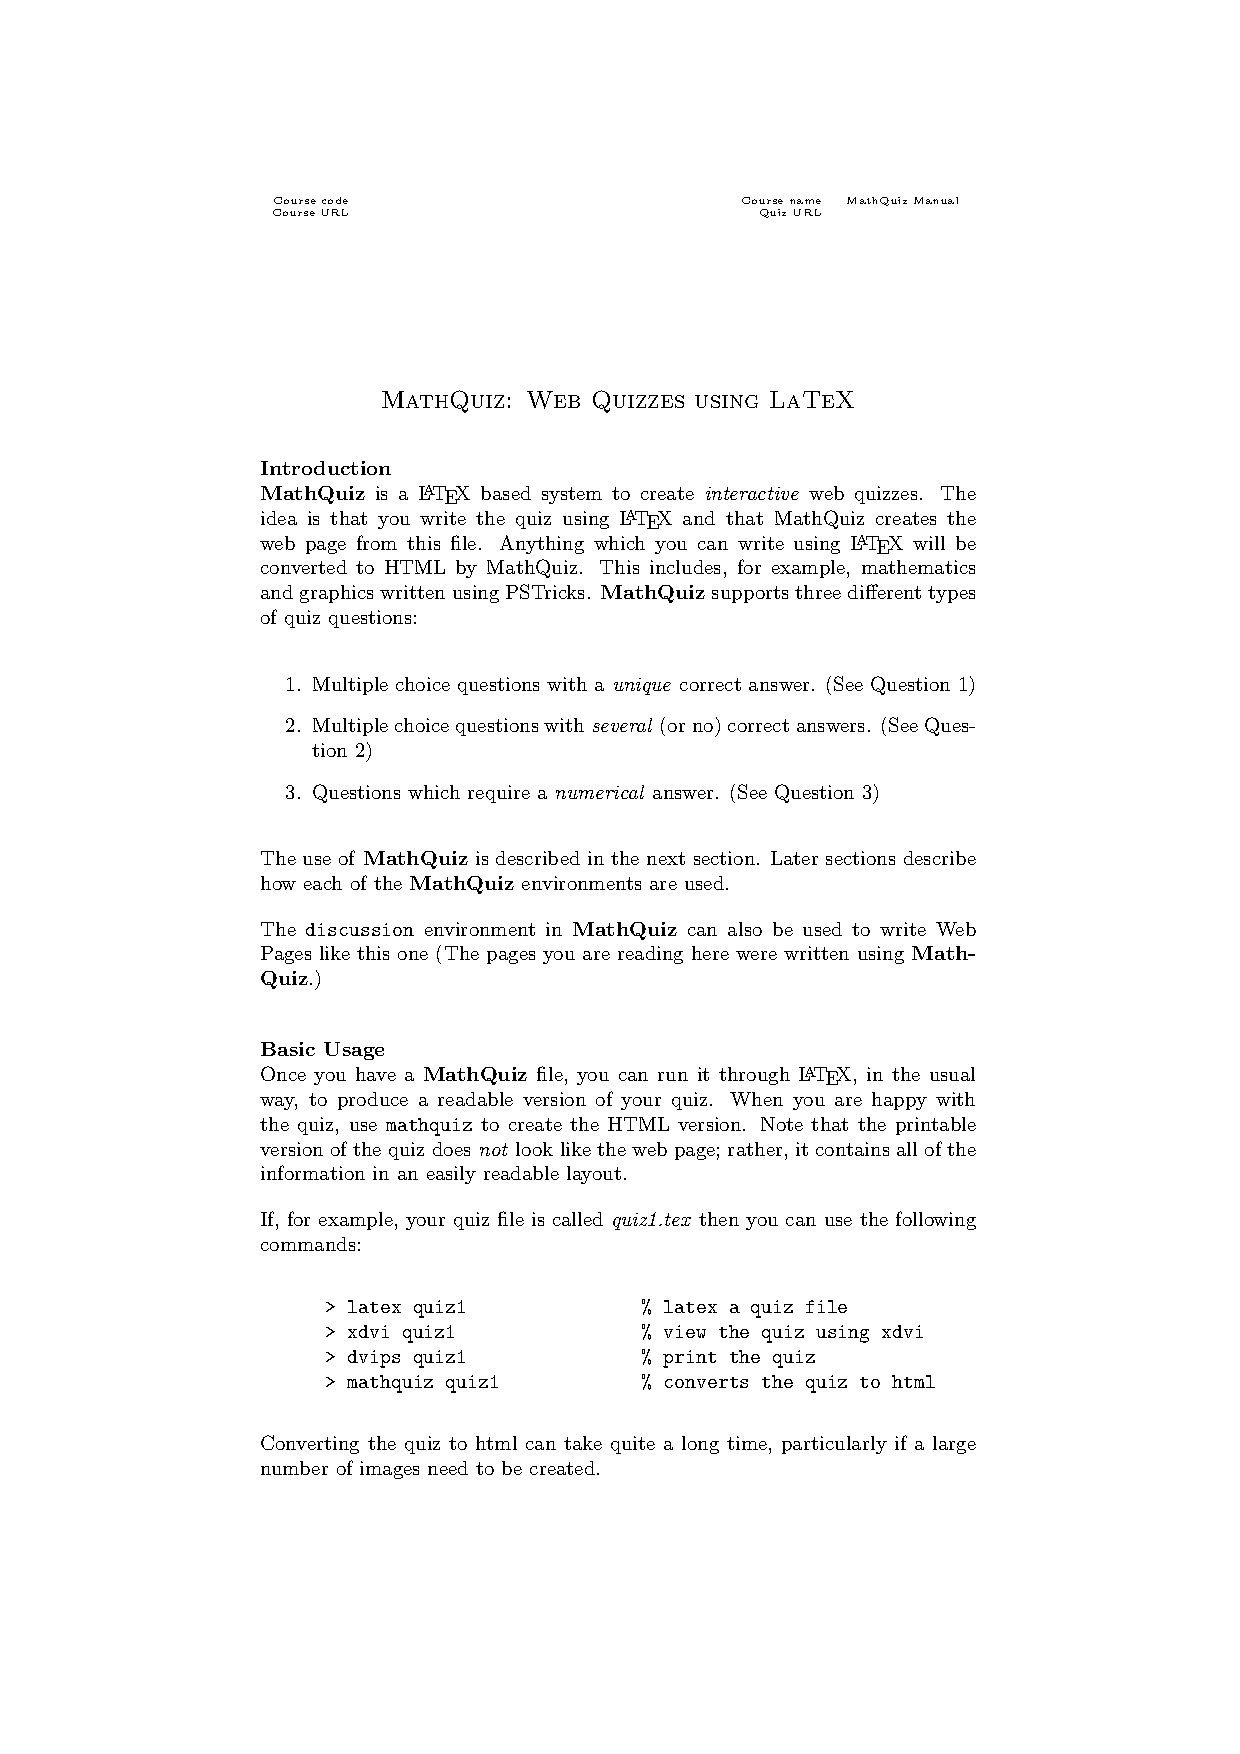
\includepdf[pages=-]{mathquiz-manual}

\section{Licence}

Copyright (C) 2013-2017

\href{https://www.gnu.org/licenses/gpl-3.0.en.html}{GNU General Public License, Version 3, 29 June 2007}

This program is free software: you can redistribute it and/or modify it under
the terms of the GNU General Public License (GPL) as published by the Free
Software Foundation, either version 3 of the License, or (at your option) any
later version.

This program is distributed in the hope that it will be useful, but WITHOUT ANY
WARRANTY; without even the implied warranty of MERCHANTABILITY or FITNESS FOR A
PARTICULAR PURPOSE.  See the GNU General Public License for more details.


\vfil
\begin{tabular}{@{}ll}
Authors             & \mathquiz{authors}\\
Description         & \mathquiz{description}\\
Maintainer          & \mathquiz{name}\\
System requirements & python3 and \LaTeX, including \TeX 4ht and \textsc{make4ht}\\
Licence             & \mathquiz{licence}\\
Release date        & \mathquiz{release date}
\end{tabular}
\eject

\printindex

\end{document}
